% Created 2016-04-28 Thu 08:16
\documentclass[11pt]{article}
\usepackage[utf8]{inputenc}
\usepackage[T1]{fontenc}
\usepackage{fixltx2e}
\usepackage{graphicx}
\usepackage{grffile}
\usepackage{longtable}
\usepackage{wrapfig}
\usepackage{rotating}
\usepackage[normalem]{ulem}
\usepackage{amsmath}
\usepackage{textcomp}
\usepackage{amssymb}
\usepackage{capt-of}
\usepackage{hyperref}
\author{Pan An (A0134556A)}
\date{\today}
\title{Directional Dipole Model for Subsurface Scattering}
\hypersetup{
 pdfauthor={Pan An (A0134556A)},
 pdftitle={Directional Dipole Model for Subsurface Scattering},
 pdfkeywords={},
 pdfsubject={},
 pdfcreator={Emacs 24.5.1 (Org mode 8.3.4)}, 
 pdflang={English}}
\begin{document}

\maketitle
\tableofcontents


\section{Introduction}
\label{sec:orgheadline1}
Jensen et al. proposed a method for rendering the effects of 
subsurface scattering by using the Bidirectional Surface Scattering
 Reflectance Distribution Function (BSSRDF). 
Subsurface scatter- ing is caused when light scatters one
 to multiple times in a semi-translucent object,
 and is very important in a variety of different objects, such
 as milk or jade. Without this effect, rendered objects have a 
rough and hard computer generated feel to them.


This effect is simulated in a ray tracer by casting samples over the surface
 of the object and into the object. Original BSSRDF renders translucent materials 
using Monte Carlo ray tracing is computationally expensive 
due to a large number of subsurface scattering events.

This report is the implementation of an analytical model for subsurface scattering 
which captures translucency effects that are present in the reference solutions but 
remain absent with existing models. The idea is that a ray source corresponds better to 
the light that refracts through the surface of a translucent material. 



\section{Related Work}
\label{sec:orgheadline2}
Subsurface scattering(SSS), is an optical physics based machanism describing the
process of light penetrating translucent materials. Different models
have been proposed in order to produce artifitial images of real life
materials. Bidirectional reflectance distribution~\cite{} function was
introduced as a simple but efficient model for reflection of light at
the surface of objects. Jensen et. al.~\cite{} introduced an improved model:
bidirectional subsurface scattering reflection distribution
function(BSSRDF).

A list of some physical caracteristics of different materials  has been
measured in Jensen's work. Gkioulekas et. al.~\cite{} studied on the
physical characteristics of daily materials. Gkioulekas et. al. used a
series of techniques and algorithms in order to achieve a set of data
for daily materials such as wine, milk, coffee etc. Based on their
analysis we are able to achieve a better result in multimedia
rendering.

\section{Platform and Frameworks}
\label{sec:orgheadline3}

My code is running on my personal computer, the specifications is listed:
\begin{center}
\begin{tabular}{lll}
\hline
\hline
Hardware & Params & Additional\\
\hline
CPU & i7 & 4700MQ\\
GPU & NVIDIA & GTX 780m\\
RAM & 16GB & \\
DRAM & 3GB & \\
OS & Windows 7 & 64-bit\\
\hline
\end{tabular}
\end{center}

Upenn(University of Pennsylvania) has open sourced one of their \href{https://cis565-fall-2015.github.io/}{framework}  for 
global illumination and rendering. My project is based on the ray tracing framework
of Upenn. Some simplified version of the calculations are also provided for analysis of the algorithm.

\section{Theory}
\label{sec:orgheadline4}

{\it Subsurface scattering} (SS) is a physical phenomenon that naturally occurs in a wide range of natural materials.
A BSSRDF is a function $S$ between two points $\mathbf{x}_i$ and $\mathbf{x}_o$ on the surface of an object
 that describes the repation between an element of emergence radiance $dL(\mathbf{x}_o, \vec{\omega}_o)$ and an 
element of incident flux $d\Phi(\mathbf{x}_i,\vec{\omega}_i)$:

$$
S(\mathbf{x}_i, \vec{\omega}_i,\mathbf{x}_o, \vec{\omega}_o) = \frac{dL(\mathbf{x}_o, \vec{\omega}_o)}{d\Phi(\mathbf{x}_i,\vec{\omega}_i)}
$$

We can then use the BSSRDF in the general formulation of the rendering equation, obtaining:
\begin{equation}
\label{eq:eq1}
\begin{aligned}
L_o(\mathbf{x}_o, \vec{\omega}_o) &= L_e(\mathbf{x}_o, \vec{\omega}_o) + L_r(\mathbf{x}_o, \vec{\omega}_o) \\
&= L_e(\mathbf{x}_o, \vec{\omega}_o) + \int_A \int_{2\pi} S(\mathbf{x}_i, \vec{\omega}_i,\mathbf{x}_o, \vec{\omega}_o) L_i(\mathbf{x}_i, \vec{\omega}_i)(\vec{\omega}_i \cdot \vec{n}_i) d\vec{\omega}_i dA
\end{aligned}
\end{equation}

Normally the BSSRDF term is split
 into two or more additional terms  in order to achieve a better approximation of the real world,
 accounting for single and multiple scattering. In case of multiple scattering, 
i.e. when light bounces multiple times inside the material, the radiance becomes largely isotropic, and the 
whole process can be treated as a diffusion.

\vspace{0.6cm}
{\bf Directional subsurface scattering}
\vspace{0.6cm}

In Jensen's work, based on approximations of the diffusion equation, the BSSRDF $S$ is modeled as two 
points lights positioned close to $\mathbf{x}_i$, and depended on the distance between the points and the 
scattering parameters. In the model we are considering for our thesis,
 proposed by Firsvad et al., we use a dipole 
of ray sources in order to better approximate the diffusion equation.
 The derived BSSRDF describes effectively the diffusion on an infinite medium, 
so some corrections are necessary in order to take into account the boundary conditions.

\begin{figure}
\begin{center}
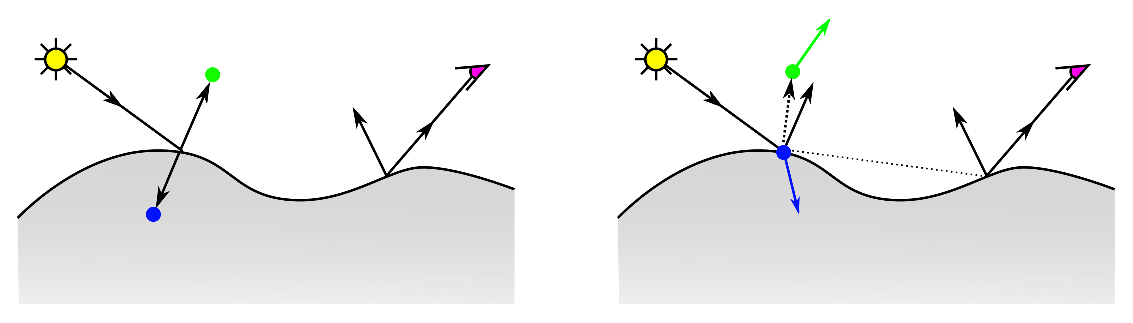
\includegraphics[scale = 0.6]{./images/comparison.eps} 

\caption{Standard dipole (on the left) versus directional dipole (on the right). }
\end{center}
\end{figure}

\vspace{0.6cm}
{\bf Approximation}
\vspace{0.6cm}

The general idea of directional dipole method is to integrate Equation \ref{eq:eq1}
 numerically. In order to do this, we need to make some assumptions. Given an emergence point $\mathbf{x}_o$.
The diffusive part of the
proposed directional dipole BSSRDF is as following:

$$
S_d({\bf x}_i, \vec{\omega_i}; {\bf x}_o)  = S'_d({\bf x}_0 - {\bf x}_i,
\vec{\omega_{12}}, d_r) - S'_d({\bf x}_0 - {\bf x}_v, \vec{\omega_v}
d_r)
$$

where $S'_d$ is the directional version of diffusive approximation.


\section{Implementation}
\label{sec:orgheadline7}
The implementation of this new method is based on the hardware that has been described before. 
I used an open source  framework provided by Upenn as the basic structure for displaying, calculation 
and error controlling. 

In order to build a platform for BSSRDF, I implemented some basic functionalities of ray tracing. As my hardware power was limited, 
I simplified a couple things in order to test faster. 
\subsection{Basic Functions}
\label{sec:orgheadline5}
Basic ray tracer model is necessary for rendering multiple objects. This GPU based path tracer with global illumination and anti-alising 
can render diffuse, perfect specular objects, transparent and subsurface scattering materials. Depth of Field was also implemented 
with some twist.

However since I did not have time to implement mesh geometry, I was not able to produce shapes other than cube and sphere.  
\subsection{Subsurface Scattering}
\label{sec:orgheadline6}
Both BSSRDF and directional dipole method were implemented. If you want to test, simply change the "BSSRDF" value of a material, then new an object into 
one of the .txt files in the scenes folder. 

Basic BSSRDF was implemented with a fast logarithmic distribution function. Directional dipole, however, was implemented with a 
Holsen sequence  generator, which is not very time efficient.

Below is an example of comparison between BSSRDF and directional dipole method:

\begin{figure}[htb]
\centering
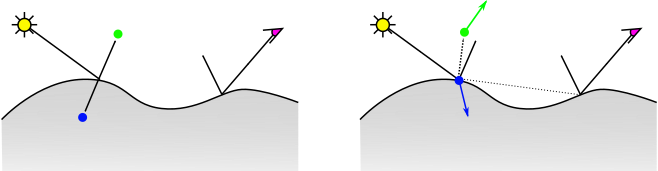
\includegraphics[width=.9\linewidth]{./img/comparison.png}
\caption{\label{fig:orgparagraph1}
This is the caption for the next figure link (or table)}
\end{figure}
\section{Results and Proposal for Further Research}
\label{sec:orgheadline8}



\section{Acknowledgements}
\label{sec:orgheadline9}
I want to thank professor Yin for offering to help with the hardware. 
The platform  that I used to develop is provided by CIS565 GPU programming course. 
Part of my report material comes from DTU github repository, will be adding license information if needed.
And special thanks to professor WengFai Wong, for the guidance of low level optimizations. 
\end{document}
